

\documentclass{beamer}
\usepackage[latin1]{inputenc}
\usepackage{minted}
\usepackage{simlab}

% Replace short paper title (inside square brackets) by our lab name
\title[Artifical Neural Networks]
{Artificial Neural Networks}
\subtitle{}
\date{\today}

%\subtitle{Include Only If Paper Has a Subtitle}

% Give the names in the same order as they appear in the paper.
% Use the \inst{?} command only if the authors have different affiliation.
% Names inside square brackets will appear at the bottom of each slide.
\author[Mitchell Corbett/Matthew Galbraith]{Mitchell Corbett and Matthew Galbraith}



% Uncomment this if you want the table of contents to pop up at the beginning of
% each subsection:
%\AtBeginSubsection[] {
%  \begin{frame}<beamer>
%  \frametitle{Outline}
%  \tableofcontents[currentsection,currentsubsection]
%  \end{frame}
%}

\begin{document} 
 
% If you wish to uncover everything in a step-wise fashion, uncomment the
% following command: 
%\beamerdefaultoverlayspecification{<+->}
\maketitle


% Comment the following lines if you wish to hide frame number
\expandafter\def\expandafter\insertshorttitle\expandafter{%
  \insertshorttitle\hfill%
  \insertframenumber\,/\,\inserttotalframenumber}

\begin{frame}
  \frametitle{Outline}
  \tableofcontents[pausesections]
  % You might wish to add the option [pausesubsections] as well.
\end{frame}

%---------------------------------------------------------------------- SECTION
\section{Introduction to ANN}
\begin{frame}
\frametitle{What is a Neural Network?}

\begin{itemize}
	\item What is a Neural Network?
    
\end{itemize}
\end{frame}
\subsection{Biological Inspirations}
\begin{frame}
\frametitle{Biological Inspirations}
\begin{itemize}
	\item In Biology, the Neuron is a fundamental unit of the Central Nervous System. It contains 3 parts. The Cell Body, Dendrites, and an Axon.
	\begin{itemize}
		\item The Cell Body contains the essential parts of the cell
		\item Dendrites are short fibers that receive signals.
		\item The Axon is a long projecting branch which sends signals. It can branch in to many other cells.
\end{itemize}
\end{itemize}
\end{frame}
\begin{frame}
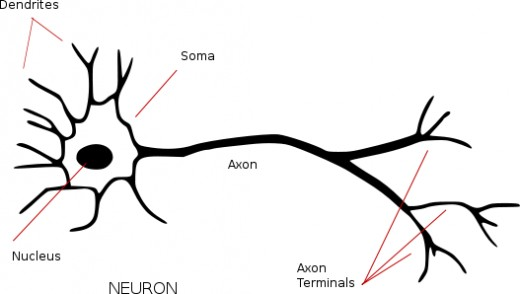
\includegraphics[width = 325px]{neuron.jpg}
\end{frame}

\subsection{Different Definitions}
\begin{frame}
\frametitle{DARPA NN Study}
\begin{itemize}
	\item "...a Neural Network is a system composed of many simple processing elements operating in parallel whose function is determined by network structure, connection strength and the processing performed at computing elements or nodes"
\end{itemize}
\end{frame}

\begin{frame}
\frametitle{Haykin (1994)}
\begin{itemize}
\item "A neural network is a massively parallel distributed processor that has a natural propensity for storing experiential knowledge and making it available for use."
\end{itemize}
\end{frame}
\subsection{Applications}
\begin{frame}
\frametitle{Applications}
Classification Problems:
\begin{itemize}
\item  Character Recognition
\item Labelling images
\end{itemize}
Regression:
\begin{itemize}
\item Recognize facial keypoint
\item Image Processing
\end{itemize}
\end{frame}

\begin{frame}
\begin{itemize}
\item With that, let's dive in!
\end{itemize}
\end{frame}
\subsection{Model of an "Artificial" Neuron}
\begin{frame}
\frametitle{What the heck is a Neuron}
\begin{itemize}
	\item We need to discuss how we can model a Neuron computationally. 
    \item A basic neuron has 3 key components. \textbf{Synapses}, an \textbf{Adder}, and an \textbf{Activation Function}.
\end{itemize}

\end{frame}

\begin{frame}
\frametitle{Components of a Basic Neuron}
\begin{block}{Synapses}
Synapses or "Links"  each have a weight assigned to them. If we have an input signal coming into a neuron, we will want to weight them differently.
\end{block}
\begin{block}{Adder}
Used for summing the input signals which have been weighted. This is also called a Summing Junction.
\end{block}

\begin{block}{Activation Function}
Used to limit the output of a neuron. Essentially, the activation function  requires that a sufficiently strong output is reached. This is very similar to the neurons in our brains, which fire or activate in response to a change in electrical charge.
\end{block}

\end{frame}

\begin{frame}
\frametitle{Activation Functions}
There are a few different choices for activation functions. Certain ones will lead to different models. 
\begin{block}{Threshold function}
A function that is 0 or 1 depending on the sign of the input. 
\end{block}
\begin{block}{Piecewise linear}
An approximation of non-linear behavior:


$
   \phi(v) \left\{
     \begin{array}{ll}
       1 &  v \geq \frac{1}{2}\\
       v & \frac{1}{2}>v>-\frac{1}{2}\\
       0 &  v \leq -\frac{1}{2}\
     \end{array}
   \right.
$
\end{block}
\end{frame}


\begin{frame}
\frametitle{Activation Functions}
\begin{block}{Sigmoid Function}
The typical choice for activation. It has the desirable property of being continuous and strictly increasing, making it a good fit for an activation function. 


$\phi(v) = \frac{1}{1+exp(-v)}$

$tanh(v_i)$ 
is a similar function that fits this description.
\end{block}
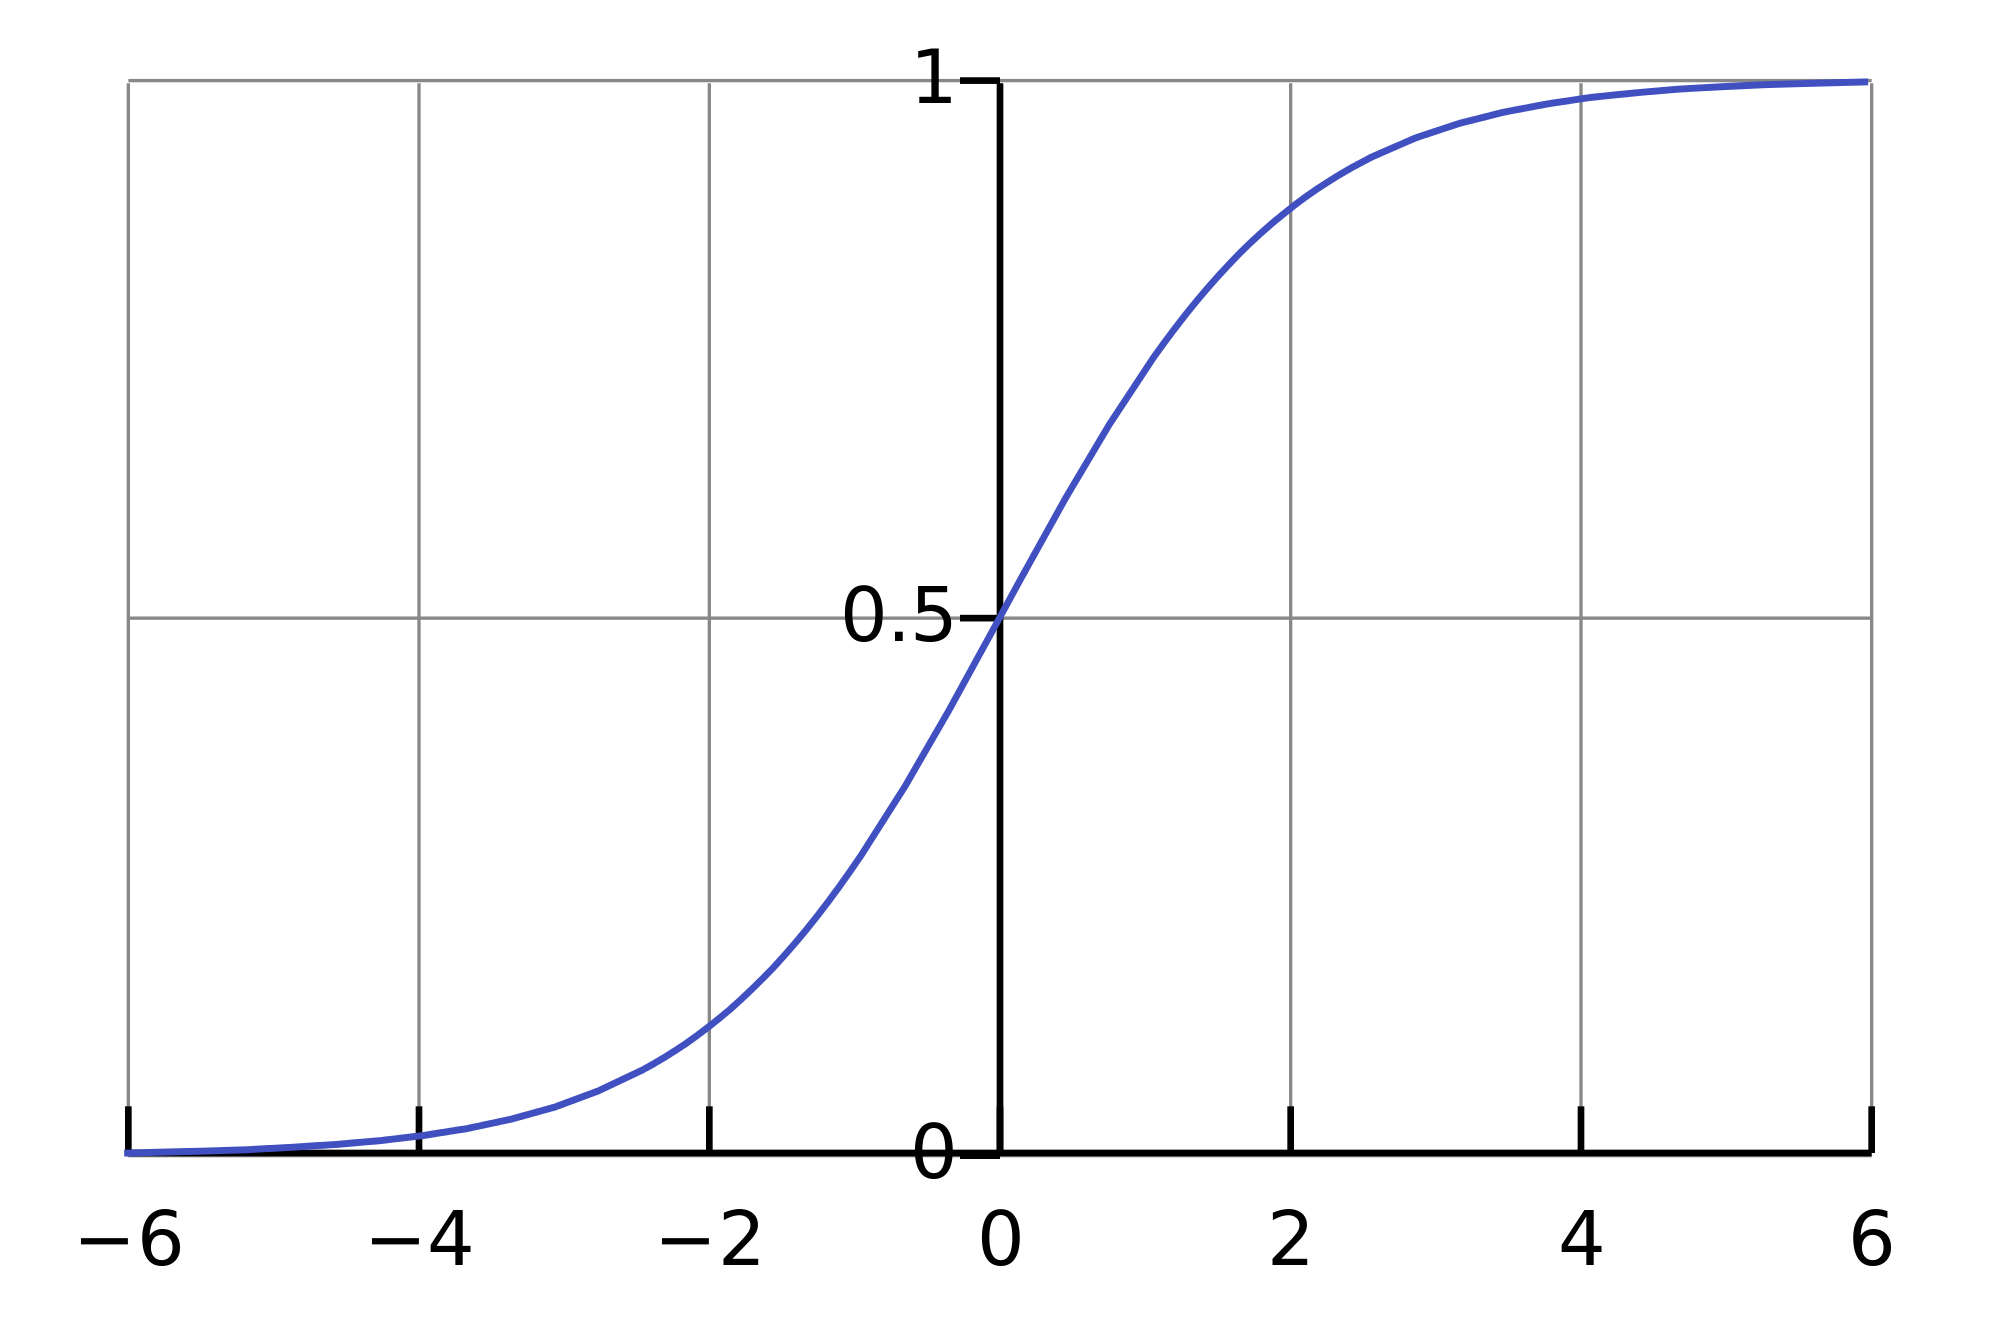
\includegraphics[width = 175px]{sig.png}
\end{frame}

\begin{frame}
\frametitle{Other Components of a Basic Neuron}
We can introduce a parameter to the sigmoid function, to control the steepness, but what if we wish have a stronger output.
\begin{block}{Bias}
The Bias increases the net output of the activation function, effectively shifting the output.
\end{block}

\end{frame}

\begin{frame}
\frametitle{Neuron Output}
Given the inputs, and defined weights, 
$$v_k=\Sigma_{j=1}^{m}w_{kj}x_j$$ is the linear combination of weighted inputs, as determined by the Adder, or Summing Junction.

$$y_k = \phi(v_k+b_k)$$ is then the outgoing signal from the neuron where $b_k$ is the bias.


\end{frame}
\begin{frame}
\frametitle{A basic Neuron}
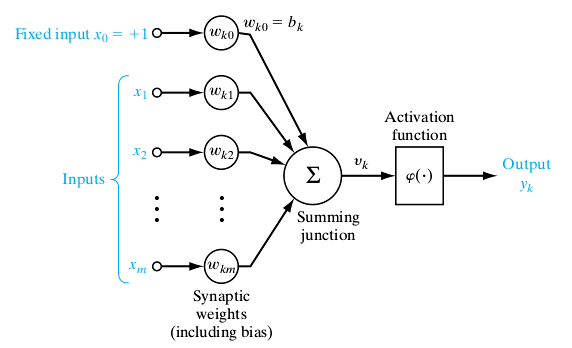
\includegraphics[width=300px]{neurond.png}
\end{frame}

\section{Feed-Forward Neural Networks}


\subsection{Single Layer Perceptron}
\begin{frame}
\frametitle{Single Layer Perceptron}
\begin{itemize}
\item We now have the terminology to examine our first Neural Network! The Single Layer Perceptron! Yay!

\item A Single Layer Perceptron (SLP) is a binary classifier that maps an input to a binary value.
\item SLP is a single neuron, all on its own, using the Threshold function for activation.
\end{itemize}
\end{frame}

\begin{frame}
\frametitle{Single Layer Perceptron}
Mathematically, we define the SLP (Single-Layer Perceptron as follows:

\begin{block}{SLP}
The SLP is a function from $R^n->\{0,1\}$ such that:
$$
   f(x) \left\{
     \begin{array}{ll}
       1 &   if \:  w\cdot x+b >0\\
       0 &  otherwise
     \end{array}
   \right.
$$
Where  $w$ is the weight vector, $\cdot$ refers to the dot product and $b$ is the bias.
\end{block}
\end{frame}

\subsection{Learning in the SLP}
\begin{frame}
\frametitle{Single Layer Perceptron - Learning}
\begin{block}{Definitions/Terminology}
\begin{itemize}
\item $y=f(\textbf{x})$ is the output 
\item $D={(x_1, d_1),\dots,(x_s,d_s)}$ is the training set of s samples where $x_i$ is the input vector, and $d_j$ is the desired output. 
\item As part of the input, we will represent the bias as a constant input , so $x_{j,0}=1$ which has a corresponding weight, so we can train it.
\item $w_i(t)$ is the weight vector corresponding to the ith input at time $t$. 
\item Also define a learning rate $0<\alpha\leq 1$ which will dictate how much our weights can change with each update.
\end{itemize}
\end{block}
\end{frame}

\begin{frame}
\frametitle{SLP Convergence}
\begin{itemize}
\item The  data in question must be linearly separable. By this we mean the existence of a hyperplane "Decision boundary" in which the two classes can be split apart.
\item This plane will be where $$\Sigma w_ix_i + b = 0 $$
\item The challenge is determining what the weights should be for the decision boundary to be correct.
\item It's easy to see that this model is incapable of describing a non-linear decision boundary
\end{itemize}
\end{frame}

\begin{frame}
\frametitle{SLP Convergence}
\begin{itemize}
\item In fact, if the data is linearly separable, then it is guaranteed to converge.

\item There is also an upper bound to the number of weight updates.$$O(R^2/\gamma^2)$$
Where R is the maximum norm of an input vector, and $\gamma$ is the margin of the hyperplane
\end{itemize}
\end{frame}

\begin{frame}{References}
\begin{itemize}
\item http://www.teco.edu/~albrecht/neuro/html/node16.html
\item Haykin, S. (1999), Neural Networks: A Comprehensive Foundation, NY: Macmillan.
\item  Novikoff, A. B. (1962). On convergence proofs on perceptrons. Symposium on the Mathematical Theory of Automata, 12, 615-622. Polytechnic Institute of Brooklyn.
\item DARPA Neural Network Study (U.S.). 1988. DARPA Neural Network Stdy. Widrow, Morrow, and Gschwendtner (Eds.). AFCEA Intl.

\end{itemize}
\end{frame}


\begin{frame}
\frametitle{Smooth Transition}
And with that... It's off to Matt!
\end{frame}

\end{document}

